%%%%%%%%%%%%%%%%%%%%%%%%%%%%%%%%%%%%%%%%%%%%%%%%%%%%%%%%%%%%%%%%%%%%%%%%%%%%%%%%
%2345678901234567890123456789012345678901234567890123456789012345678901234567890
%        1         2         3         4         5         6         7         8

\documentclass[letterpaper, 10 pt, conference]{ieeeconf}  % Comment this line out if you need a4paper
\usepackage{graphicx}
\usepackage{subcaption}
\usepackage{cite}
\usepackage{multicol}
\usepackage{url}
\usepackage{textcomp}
\usepackage{textgreek}
\usepackage{fixltx2e}


%\documentclass[a4paper, 10pt, conference]{ieeeconf}      % Use this line for a4 paper

\IEEEoverridecommandlockouts                              % This command is only needed if 
                                                          % you want to use the \thanks command

\overrideIEEEmargins                                      % Needed to meet printer requirements.

% See the \addtolength command later in the file to balance the column lengths
% on the last page of the document

% The following packages can be found on http:\\www.ctan.org
%\usepackage{graphics} % for pdf, bitmapped graphics files
%\usepackage{epsfig} % for postscript graphics files
%\usepackage{mathptmx} % assumes new font selection scheme installed
%\usepackage{times} % assumes new font selection scheme installed
%\usepackage{amsmath} % assumes amsmath package installed
%\usepackage{amssymb}  % assumes amsmath package installed

\title{\LARGE \bf
Cycloidal Geartrain In-Use Efficiency Study
}

\author{Logan C. Farrell$^{1}$, James Holley$^{2}$, William Bluethmann$^{3}$, and Marcia K. O'Malley$^{4}$% <-this % stops a space
\thanks{$^{1}$Logan Farrell is with the Department of Mechanical Engineering at Rice University and NASA: Johnson Space Center.
		{\tt\small Logan.C.Farrell@NASA.gov}}%
\thanks{$^{2}$James Holley is with the Department of Mechanical Engineering at Rice University and NASA: Johnson Space Center.}%
\thanks{$^{3}$William Bluethmann is the project manager for rovers at NASA: Johnson Space Center.}%
\thanks{$^{4}$Marcia O'Malley is on the Faculty in the Department of Mechanical Engineering, Rice University, Houston, TX}%
}


\begin{document}



\maketitle
\thispagestyle{empty}
\pagestyle{empty}


%%%%%%%%%%%%%%%%%%%%%%%%%%%%%%%%%%%%%%%%%%%%%%%%%%%%%%%%%%%%%%%%%%%%%%%%%%%%%%%%
\begin{abstract}

Currently, Harmonic Drives are the go-to speed reducer for robotic applications where a high reduction in a small package is required. However, cycloidal drives can also fit this mold with the ability to customize a high reduction drive that can carry high torque in a small package. These compact style cycloidal drives have been well studied in the theory and simulation for their performance, but very little data is available on their actual performance over time. This study used a cycloidal drive designed for a robotic application and ran it through 37K (TODO) cycles over 80 (TODO) hours of testing to determine burn-in time, efficiency curves, and efficiency profiles over time to determine its comparison to a Harmonic Drive in-use. The study finds that substantial burn-in time may be required for steady-state performance, but peak efficiencies of 77\% can be achieved. Also, the efficiency is dependant on the torque through the actuator, contrary to multiple previous studies. This work demonstrates a cycloidal drive in a robotic application that is comparable to a Harmonic Drive, suggesting the application of cycloidal drives could grow tremendously in robotic designs. 

\end{abstract}


%%%%%%%%%%%%%%%%%%%%%%%%%%%%%%%%%%%%%%%%%%%%%%%%%%%%%%%%%%%%%%%%%%%%%%%%%%%%%%%%
\section{INTRODUCTION}
As robotic applications flourish in our modern world, there is an increasing need for  high reduction, high torque, and low backlash actuator systems. These actuators are present in all types of robotic equipment. This need is true in space flight applications as well. A notable recent example includes the Curiosity rover from NASA's Jet Propulsion Laboratory \cite{curiosity} that uses primarily Harmonic Drives. Currently, Harmonic Drives are the primary reduction method when high ratio and compact design are required. These reducers come in limited reduction ratio options, and can grown quite heavy to withstand the high torque applications. This leads to the need for an alternative high reduction, compact drive system for these applications. 

\subsection{Cycloidal Drive Motivation}

Cycloidal drives are potentially an apt replacement for these Harmonic Drives as they can offer large a large reduction in a small package. They provide some distinct advantages as well in situations where small backlash is acceptable, such as their ability to be customized into the system directly and are made of relatively easy to manufacture parts, unlike a Harmonic Drive. In addition, the torque to weight ratio typically higher for cycloidal drives of this style, the cycloid presented in this work is X (TODO) kg and a comparable Harmonic Drive is 19.8kg.
However, there is insufficient data available for the true efficiency and characteristics of these drives. The primary contribution of this research shows the efficiency of a cycloidal drive system designed for a robotic application. This is done through an extended drive cycle test for burn-in to steady state performance over 37K (TODO) revolutions through 80 (TODO) hours and efficiency testing over the torque and speed range of this system. 

   \begin{figure}[!b]
      \centering
      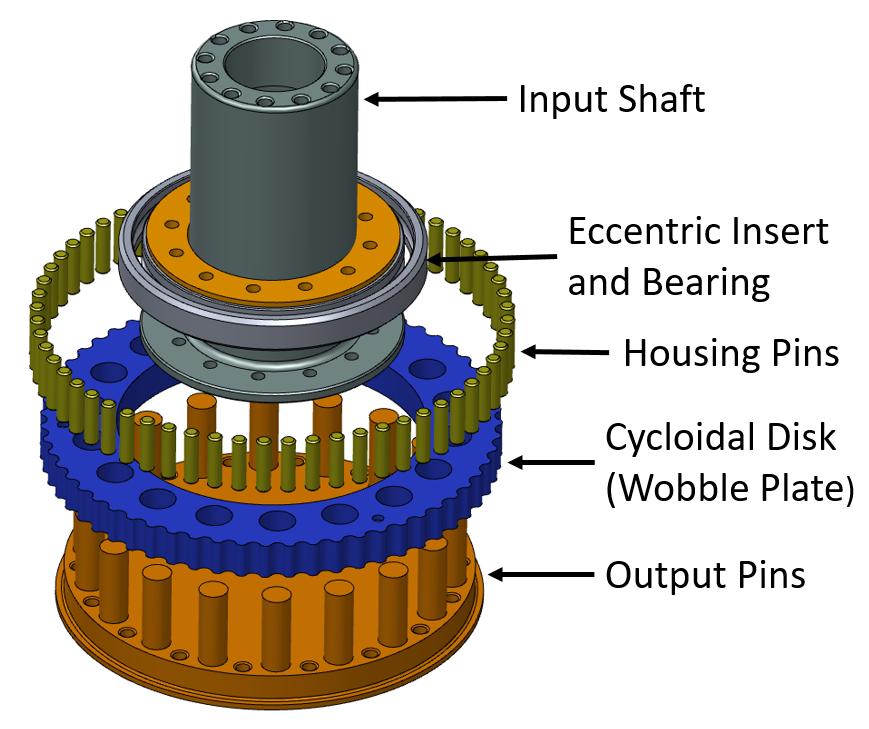
\includegraphics[width=0.50\linewidth]{cycloid_cartoon_v2}
      \caption{Simple rendering of the key elements that create a cycloidal drive. A drive shaft spins a cycloidal disk (wobble plate) via an eccentric circle. The wobble plate reacts against the housing pins to create a counter-rotation, harnessed by the output pins.}
      \label{cycloid_cartoon}
   \end{figure}
   
\subsection{Cycloidal Drive Background}
Cycloidal drives were proposed as early as 1956 by Botsiber and Kingston \cite{1956}. The premise of this design leverages a plate, referred to as the wobble plate, with lobes interacting with pins in the housing designed using trochoidal motion being spun on an eccentric shaft with a bearing. This induces a counter-clockwise motion of the plate and this is harnessed with the interior pins as the output of the mechanism. This basic layout can be seen in Fig \ref{cycloid_cartoon}. This geartrain design has been used in industry for high torque, high shock load applications for many years\footnote{http://www.nabtescomotioncontrol.com/engineering.php}. However, in many of these applications, all of the interacting surfaces like the housing pins and output pins use needle roller bearings to transmit load. This allows for higher efficiency and load carrying capability but it also increases mass and size for a given design need. In the robotic industry, groups are striving to reduce the mass and size of these actuators while still achieving the high reduction and load capabilities. The primary method to do this is to eliminate many of the rolling elements at the interaction points between the wobble plate, housing pins, and output pins. This allows for very compact and strong designs to be considered but leaves the potential for larger losses and lower system lifetime. 

Many works have been presented on the subject of the theoretical design of these cycloidal drives \cite{on_the_lobe} \cite{hwang_hsieh}, designing with machine tolerances \cite{design_and_application}, contact and stress analysis \cite{li}, and performance characteristics such as torque ripple and backlash \cite{hsieh_traditional} \cite{hsieh_dynamics}. Please see See Section \ref{design} for details. These works lay a solid foundation to a designer with the equations and design considerations to take while designing a cycloid. However, there has been very little work done in the area of in-use characteristics aside from the theoretical calculations and models. 

Many of researchers have explored and presented calculations for the efficiency, Malhorta and Parameswaran calculated between 98\% and 88\% efficiency for designs \cite{Malhorta} and Sensinger predicted 95\% \cite{unified_approach}. Later, Sensinger and Lipsey performed a short one and a half hour study on the efficiency of a cycloid test article \cite{cycloid_vs_harmonic} showing efficiencies in the 40\% range for fused roller designs, and 60\% for pin designs. Fused rollers designs machine the roller designs manufacture the ring pins are part of the housing, pin roller designs insert pins into holes to allow relative motion during contact. In addition, Hsieh verified the stress present in the drives in simulation and in use and demonstrated lower stress levels and torque ripple when using fused rollers \cite{hsieh_dynamics}. 

The aim of this work is to utilize a custom cycloid design for a NASA rover application and show the in-use efficiency characteristics over a more extended duration test. First, the authors will detail the actuator design in Section \ref{design}. Second, a description of the experimental setup and procedure is provided in Section \ref{methods}. Finally, the results and analysis of this high torque actuator and its implications are presented and discussed in Section \ref{results} and Section \ref{discussion}. 

NOTE TO O'MALLEY: Should I put my contribution statement here or leave it higher in the document?

\section{CYCLOID DESIGN} \label{design}

\begin{table*}[t]
\caption{Designed Duty Cycles for System}
\label{duty_cycle}
\begin{center}
\begin{tabular}{|c||c||c| |c| |c|}
\hline
Time Used & Output Torque (Nm) & Output Speed (RPM) & Actuator Torque (Nm) & Actuator Speed (RPM)\\
\hline
5\% & 2440 & 6.8 & 554.7 & 33.9\\
\hline
20\% & 1627 & 6.8 & 369.8 & 33.9\\
\hline
60\% & 542 & 15.3 & 123.3 & 76.3\\
\hline
15\% & 135 & 15.3 & 30.8 & 76.3\\
\hline
\end{tabular}
\end{center}
\end{table*}


   
In 2007 and 2008, NASA developed a manned rover prototype for planetary surfaces for future missions \cite{rover}. This robotic vehicle is made up of six independent wheel modules, each with their own propulsion, steering, and both active and passive suspension. In 2014, a new prototype wheel module was designed and created to analyze new potential technologies that could be used in these application. In the new design layout, it was possible for the propulsion wheels to counter-rotate against the steering and put large shock loads into the steering system.These requirements for a high load, compact package, high shock load, and tolerance of backlash lent itself to the selection of a cycloidal drive for the steering actuator. This actuator was then selected for the continued testing presented in this paper. The prototype wheel module layout can be seen in Fig \ref{acuator_layout}.

NOTE FOR O'MALLEY: Does this figure add anything other than length? 
   \begin{figure}[t]
      \centering
      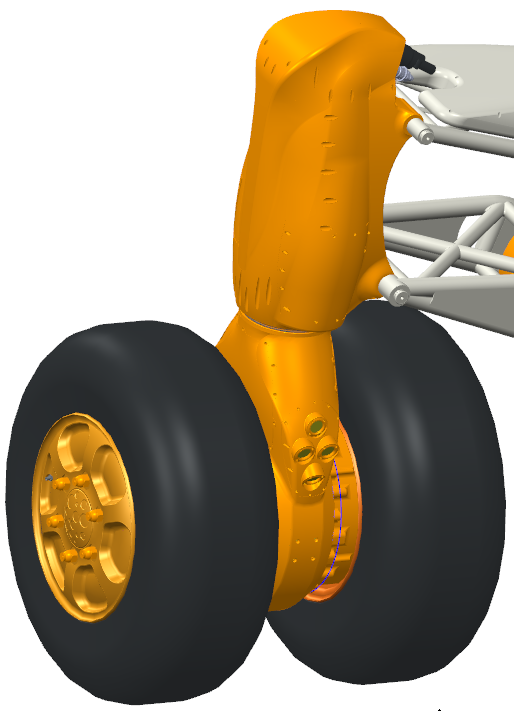
\includegraphics[width=0.50\linewidth]{wheel_module_CAD}
      \caption{CAD model of rover wheel module prototype. Suspension arms hold the steering column. Each wheel has an in-wheel propulsion motor.}
      \label{cycloid_cartoon}
   \end{figure}
   
Based on the load cases the actuator was required to output a stall torque of 2,440 Nm (1800 ft-lb) with a max output speed of 1.57 rad/s (90 deg/s) at 1,626 Nm (1200 ft-lb). The required torque speed data points can be seen in Table \ref{duty_cycle} with an assumed loss of 88\% chosen based on the available literature. The actuator layout for the vehicle placed the motor and cycloid off center of the steering axis with an additional 5:1 reduction into the steering column, thus decreasing the torque needed for the cycloid output, but increasing the potential shock loading. 

Many sources have laid out the design parameters for these drives and the equations are provided below for completeness. Shin and Kwon \cite{on_the_lobe} presented the mathematical definition of the cycloid profile

\begin{equation} \label{eq:1}
C_x = R cos\phi -R_r cos(\phi + \psi) - e cos((Z_1 + 1)\phi) 
\end{equation}
\begin{equation} \label{eq:2}
C_y = -R sin\phi + R_r sin(\phi + \psi) + e sin((Z_1 + 1)\phi) 
\end{equation}
\begin{equation} \label{eq:3}
\psi = tan^{-1} \lbrack\frac{sin(Z \phi)}{cos(Z \phi) - R / (e(Z + 1))}\rbrack 
\end{equation}

where \textphi\ is the angle of the input shaft and \textpsi\ is the angle of contact between the outer pin and the cycloid lobe. 

Using both the formula for the reduction in diameter of the cycloid disk to account for machine tolerances \cite{machine_design} \cite{design_and_application} as well as Ye et al.'s formula for calculating the limit of undercutting \cite{ye}, the allowable sizes of the profiles and pins can be determined. Sensinger \cite{unified_approach} laid out simple equations for calculating stress on the lobes and pins that has been further modelled and studied by others. The force on the cam for calculating the bearing load with eccentricity e, ratio Z , and torque T is

\begin{equation} \label{eq:4}
F_{cam} = \frac{T}{e Z}.
\end{equation}

The simplified stress equations where R and R\textsubscript{r} are defined above, t is the contact thickness, and b is the width of contact determined by (\ref{eq:7}) and (\ref{eq:8}) are

\begin{equation} \label{eq:5}
F = \frac{T}{R - R_r}
\end{equation}
\begin{equation} \label{eq:6}
\sigma = \frac{2F}{\pi b t} (3 + 4v^2)
\end{equation}
\begin{equation} \label{eq:7}
b = \sqrt{\frac{4F (v-v_1^2) /E_1 + (1 - v_2^2)/E_2}{\pi l (1/R_1 + 1/R_2)}}
\end{equation}
\begin{equation} \label{eq:8}
R_2 = \frac{(R-eZ - e)^3}{R-e(Z-1)^2} - R_r.
\end{equation}

   \begin{figure}[!b]
      \centering
      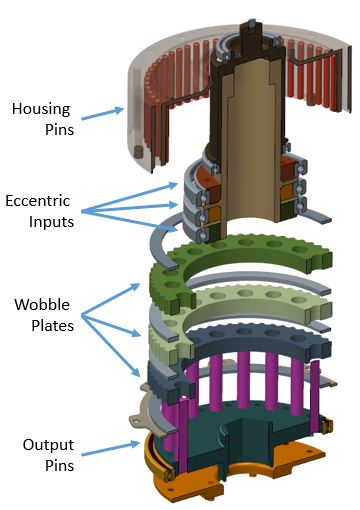
\includegraphics[width=0.75\linewidth]{exploded_labeled}
      \caption{Exploded view of the cycloidal reducer. Three wobble plates are driven by the input shaft with 120\textdegree\ offsets. The ring pins are are free pins inserted in the housing. The output has pins that run through all three wobble plates to harness the counter-rotation for the drive output.}
      \label{cycloid_exploded}
   \end{figure}
   
The stress calculations and trading of overall size and ratio led to a necessary plate thickness of 3.81cm (1.5in) ( (TODO: Verify). Instead of a single large plate however, three wobble plates were selected to split the load on the central input shaft across three bearings as well as to build in natural balance for the actuator. If a single plate is used, a counterbalance must be added to avoid extreme vibration. In this case, the three plates were offset 120\textdegree\ to balance these loads and vibration. This adds additional stack height to the system to allow separation between the plates. This arrangement allows the large design loads to be able to be handled by the system. The exploded view of this design can be seen in Fig \ref{cycloid_exploded}. 

The actuator uses a Parker Frameless Kit Motor, model K089200-7Y with no hall effect sensors and is commutated using a Renishaw RM-44 magnetic incremental and absolute position sensor. The final reduction is 59:1 going before into the final 5:1 output gear. The system is commutated using the delta hysteresis commutation scheme \cite{electric_machines} using velocity control. 

\section{EXPERIMENTAL METHODS}\label{methods}

   \begin{figure}[!b]
      \centering
      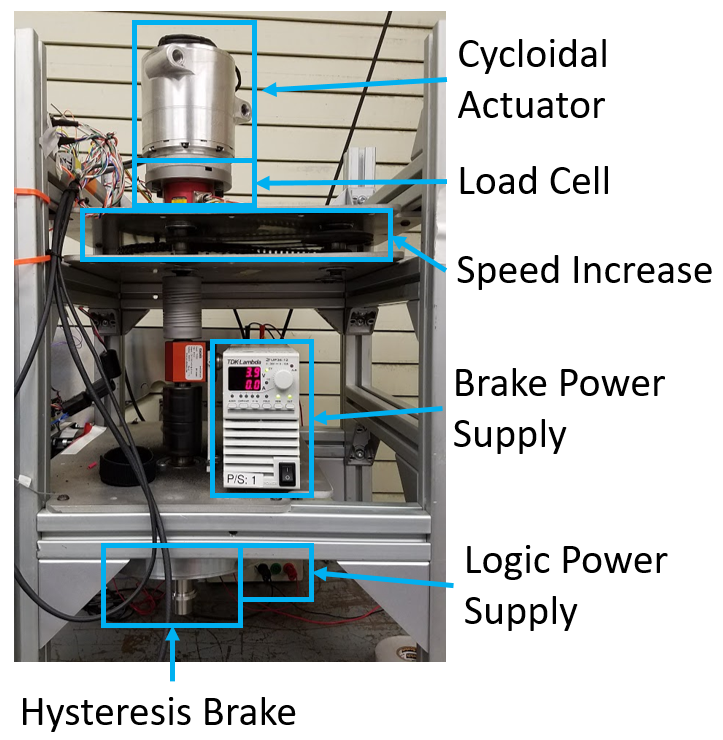
\includegraphics[width=0.75\linewidth]{test_stand}
      \caption{Experimental Test Setup. The cycloid actuator is mounted to structure via the load cell. There is a speed increase so the brake can generate enough torque on the system. Not pictured is the controlling computer, motor driver, and high voltage supply.}
      \label{test_setup}
   \end{figure}
   
The primary goal of this testing and validation was to demonstrate in-use efficiency and characteristics of a cycloid designed for a robotic application as compared to its harmonic drive counterpart that would normally be selected for these applications. Previously, the most extensive testing in Sensinger and Lispey ran for approximately one and a half hours \cite{unified_approach} using a simple, general design, whereas this actuator was designed for specific robotic use and has been run for over 37K (TODO) cycles over 80 (TODO) hours. 

The test setup is shown in Fig \ref{test_setup}. The actuator is mounted directly to a Futek TF600 5000inlb load cell to measure direct output torque of the actuator. This is read through a conversion board into the motor driver. A verification of torque readings was completed using a calibrated torque wrench to ensure accuracy of the conversion. The motor output runs through a 36:1 (TODO) speed increase via 3 chain stages that then inputs into a Magtrol HB-1750 hysteresis brake that is powered using a separate 24V Lambda-TDK power supply controlled by the computer. The motor is driven with a custom motor driver powered from a 12V Lambda-TDK power supply for logic power, and a 300V, 5A TDK-Lambda power supply for motor power. The motor driver is commutating using the incremental encoder and an index pulse and is reading the RMS phase current, motor and bridge temperatures with thermistors, motor velocity, and the torque measurement from the custom conversion board. These values are then streamed to a controlling computer that is also monitoring the high voltage supply and recording voltage and current to determine input power to the system. 

Due to the tightly integrated actuator design, the motor and cycloid cannot be separated to purely isolate the losses in the cycloid. Instead, the efficiency map of the motor over its torque and speed range was provided by Parker Motors. For calculation purposes, this table is used as a lookup table for efficiency of the motor given the current motor velocity and rms input current. While this does generate a level of uncertainty in the data, these motors are mass manufactured and defects are assumed to be small. Therefore, the error in the motor efficiency map is assumed to be small and would not influence the perceived trends and results. The efficiency losses in the motor driver can be characterized primarily by the TODO -- switching electronics and which are rated as 97\% efficient in this voltage and current range -- TODO. 

   \begin{figure}[!b]
      \centering
      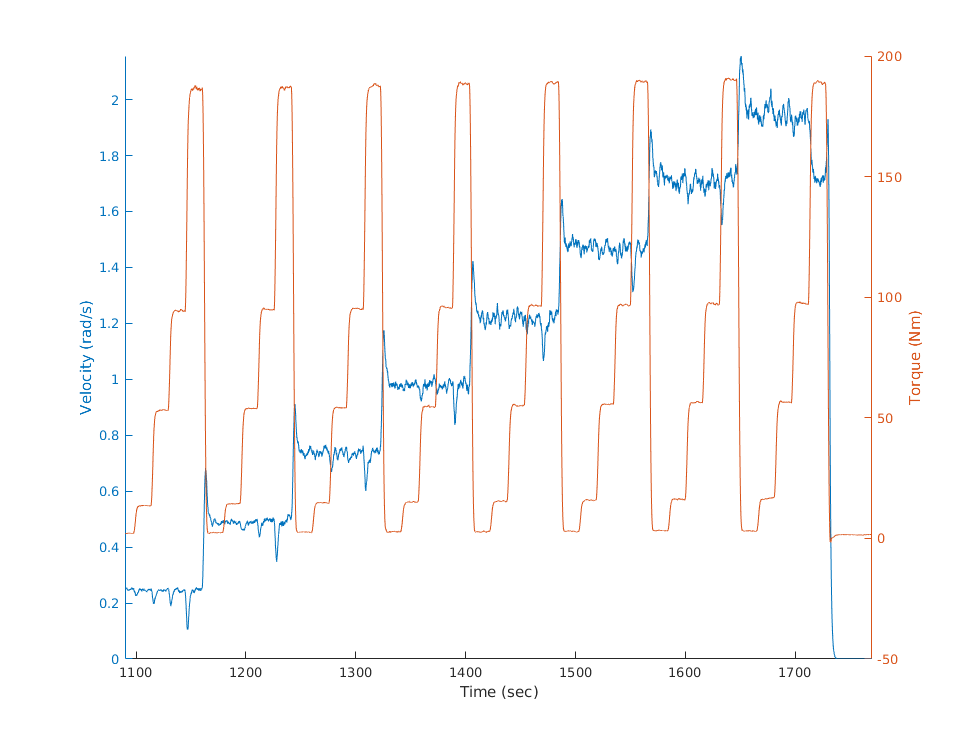
\includegraphics[width=\linewidth]{eff_test_profile_v3}
      \caption{Testing profile for efficiency. At each speed step, torque is ramped up through five different levels, then the speed is increased. At the last step, the maximum of the supply was reached so motor velocity dropped.}
      \label{eff_profile}
   \end{figure}
   
The system was tested in two separate ways, an efficiency cycle and a long term drive cycle. The efficiency cycle was run after the long term drive cycle to ensure steady state performance of the system. The efficiency test was run after a day of drive cycle testing to ensure steady state performance before cycling through a set of velocities and torques. The system steps through eight velocity steps increasing 0.25 rad/s each time. In each velocity step, the torque is ramped up and maintained for 15 seconds at values of 1Nm, 15Nm, 52Nm, 94Nm, and 189Nm. This testing profile can be seen in Fig \ref{eff_profile}. The long term drive cycle was run continuously each day for 6 to 12 hours with the duty cycles shown in Table \ref{table_2}. The total runtime of the system not including the initial checkout and verification of the actuator has been 80 (TODO) hours. 


\begin{table}[h]
\caption{Long Run Drive Cycle}
\label{table_2}
\begin{center}
\begin{tabular}{|c||c||c|}
\hline
Time (s) & Velocity (rad/s) & Torque (Nm)\\
\hline
150 & 1.0 & 0.0\\
\hline
150 & -1.0 & 0.0\\
\hline
60 & 0.5 & 26.0\\
\hline
60 & -0.5 & 26.0\\
\hline
150 & 1.5 & 10.0\\
\hline
150 & -1.5 & 10.0\\
\hline
30 & 1.0 & 50.0\\
\hline
30 & -1.0 & 50.0\\
\hline
300 & 0.5 & 18.0\\
\hline
300 & -0.5 & 18.0\\
\hline
\end{tabular}
\end{center}
\end{table}

After initial development and construction of the prototype wheel module, the test actuator was used briefly in the robot validation. The total time of use was approximately three hours. Afterwards, it was removed to be used for individual testing that is discussed in this work. During testing, the equipment available limits the maximum performance of the system below its initially designed values. The actuator was designed to be fluid cooled to allow continuous operation near and above its continuous rating of 4.3A(RMS) and 15A peak, therefore for long duration testing, the torque values were decreased to avoid thermal issues. The motor was tested to approximately 6A (RMS) during efficiency testing due to the limit of the power supply. Also, the motor driver equipment available limits the voltage to 150V, therefore the maximum speeds could not be attained. However, the nominal cycle of the actuator as seen in Fig \ref{duty_cycle} is still achievable and has been tested. 
      
   \begin{figure*}[t]
      \centering
      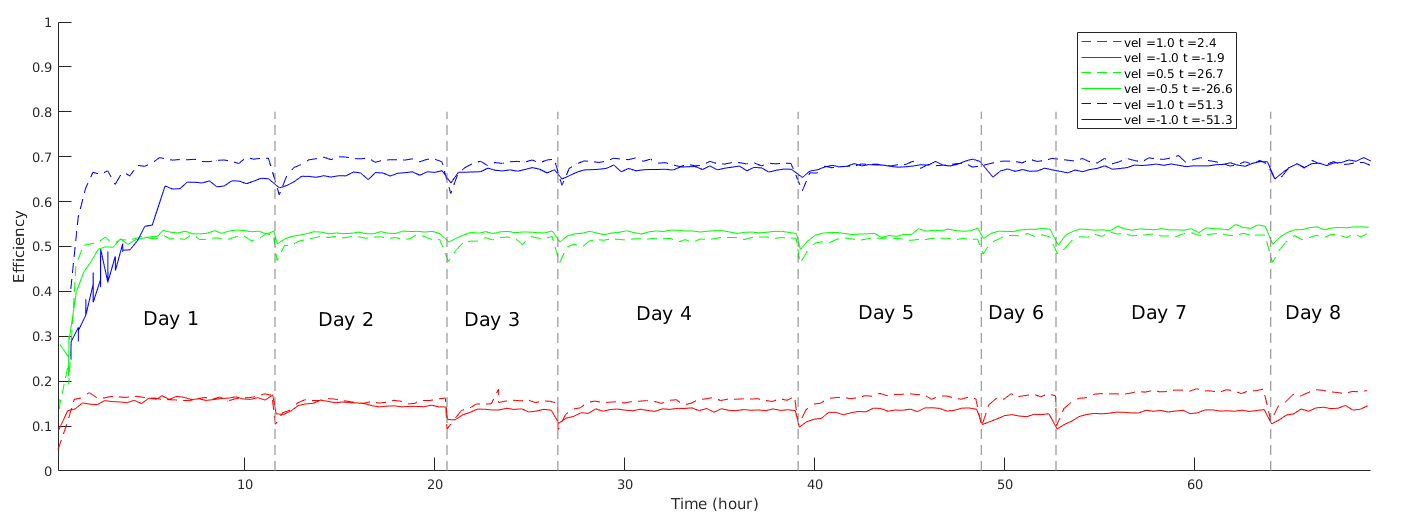
\includegraphics[width=\linewidth]{long_run_plot_v3}
      \caption{Efficiency over time for three different speed/torque profiles during the drive cycle. The forward motion can be seen with the dotted line, reverse with the solid line. At the onset of testing, visible efficiency gains are made. As each day begins, there is a clear warm-up period before steady state. TODO: add a line for start of each day}
      \label{long_run}
   \end{figure*}
   
   
\section{RESULTS} \label{results}

   \begin{figure}[t]
      \centering
      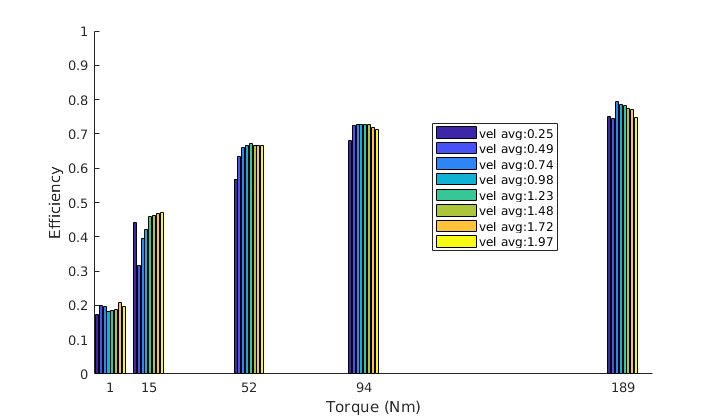
\includegraphics[width=\linewidth]{eff_test_bar_plot_v2}
      \caption{Grouping of average efficiencies at each torque step. Efficiency depends heavily on torque, and slightly on speed.}
      \label{eff_results}
   \end{figure}

Duty cycle testing was first performed on the actuator. These tests were done at lower torques to prevent the motor from overheating to allow extended duration testing. The total test time prior to these duty cycle tests were approximately 5.2 hours to bring up and check out the actuator testbed system. Once this checkout was complete, the 80 hours (TODO: put final number) of testing was done over the course of 8 (TODO) days with the drive cycle discussed in Section \ref{methods}. Three of the torque/speed combinations in forward and reverse were plotted on Fig \ref{long_run} to show the general characteristic trends seen in the actuators performance. 
   
After this duty cycle testing to prove the actuator had sufficiently broken-in and achieved steady state performance, the pure efficiency cycles were run. As discussed in Section \ref{methods}, a profile of speeds and torques were run with the actuator to show the relationship between speed, torque, and efficiency. An example of this profile can be seen in Fig \ref{eff_profile}. This profile was run three times and the results were averaged. These results can be seen in Fig \ref{eff_results}. 

\section{DISCUSSION} \label{discussion}

It is readily apparent from Fig \ref{eff_results} that the efficiency of the system is dependant on the torque through the gearbox. This contradicts previous studies that suggested that cycloidal drives have a constant efficiency across the torque range. There is also a much less pronounced relationship between the velocity and the cycloid efficiency that can be noted in the torque bands. This result suggests that the cycloid efficiency behaves more like a planetary or Harmonic Drive gearbox in its efficiency profile. A comparison of cycloid, Harmonic, and planetary efficiency profiles can be seen in Fig \ref{eff_comp}. The figure shows the efficiency for a Harmonic Drive CSG-50-80-2UH \cite{harmonic_sheet} which has a comparable ratio and torque capability to the tested cycloid and weighs 19.5kg, and a representative planetary curve \cite{planetary}. This shows that if backlash is acceptable in the system, a cycloidal drive can provide similar or better efficiency profiles to a harmonic drive while providing a potential 2x (TODO) increase in torque density.

   \begin{figure}[!b]
      \centering
      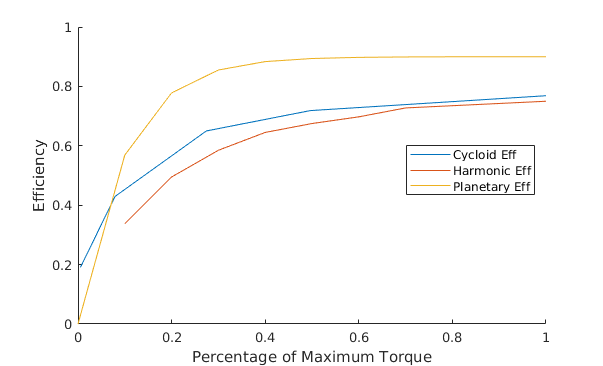
\includegraphics[width=\linewidth]{eff_comp_v2}
      \caption{Comparison of efficiency over maximum torque rating of the tested cycloid, a comparable harmonic drive, and a theoretical planetary gearset. The cycloid exhibits the same efficiency increase over torque range and has a comparable and slightly higher efficiency than the harmonic.}
      \label{eff_comp}
   \end{figure}
   
From Fig \ref{long_run} it can be observed that there was a substantial break-in time for the actuator before steady state results were achieved. In the high torque case, specifically in the reverse direction, there was an approximately linear increase in efficiency over the course of the first seven hours of duty cycle testing. This testing began after a minimum of five hours of run time spread out through many short sessions while getting the test system running. The large increase in efficiency can be noted in the other lower torque profiles as well, starting well below their final steady state values. The authors theorize that this is potentially due to break-in of the manufactured parts due to machining inaccuracies. Due to the complex interaction required of the trochoidal motion profile, slight manufacturing deficiencies could cause build-ups of stress and loss in particular points on the drive. It would make sense that these could manifest in one direction and not the other if a lobe was misshapen on the trailing edge in one direction, it would be the lead in the other, causing the additional loss. Through the first hours of testing, these materials likely wore in to each other until the contact was smooth, resulting in the more readily achieved steady state efficiencies. 

Additionally, there is a marked improvement over the first 30 minutes of runtime in the efficiency of the system. This is likely due to the grease and heat in the system. The gearbox is greased with Lucas Oil Red'N'Tacky\footnote{\url{https://lucasoil.com/products/grease/red-n-tacky-grease}} which has a viscosity index of 86 min. This was chosen because it is designed for high loads for extended periods of time in gear and sliding surface applications. Therefore, during the warm-up period as the actuator temperature increases, the viscosity decrease is likely enough to cause a notable increase in efficiency of the system. The authors leave the study of a lower viscosity grease's effect on performance for future work. 

\section{CONCLUSIONS}

This study demonstrates a cycloidal actuator with a ratio of 59:1 and three phased cycloid disks that achieves a maximum efficiency of 77\% and does not show a constant efficiency through its torque profile as suggested by previous sources. This research shows that these drives efficiencies behave very similarly to other typical reduction drives for similar applications like Harmonic Drives and Planetary gears. This actuator compares closely to its Harmonic Drive counterpart in efficiency performance. If backlash is acceptable in the system, a cycloidal drive has the distinct advantage of being customized into the housing using simple manufacturing techniques allowing tighter integration into a robotic system as well as a potential 2x torque density gain. An item of interest that has not been characterized by the community is the lifetime characteristics of these actuators and this is left by the authors for future work. Cycloidal drives of this design style are quite comparable to similar use-case drives and should be considered in high reduction applications.

\section{ACKNOWLEDGEMENTS}

The authors would like to thank the original actuator designer, Mason Markee for his support in the testing and research of this system.  

\addtolength{\textheight}{-12cm}   % This command serves to balance the column lengths
                                  % on the last page of the document manually. It shortens
                                  % the textheight of the last page by a suitable amount.
                                  % This command does not take effect until the next page
                                  % so it should come on the page before the last. Make
                                  % sure that you do not shorten the textheight too much.



%\begin{thebibliography}

\bibliographystyle{IEEEtran}
\bibliography{Cycloid_ICRA_Bib}


%\end{thebibliography}

   \begin{figure}[!b]
      \centering
      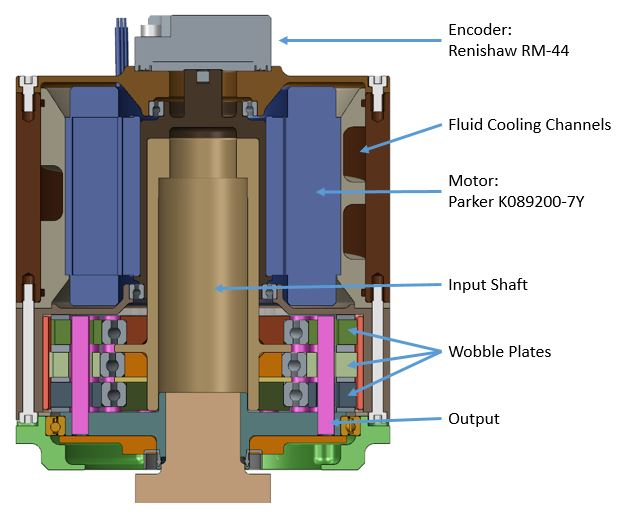
\includegraphics[width=\linewidth]{cross_labeled}
      \caption{Second option for actuator diagram. Could replace or be used in addition}
      \label{cross_labeled}
   \end{figure}


\end{document}

\begin{comment}
Abstract 7 questions 

Focus/Problem to be Solved: 
	How efficient are cycloids actually when designed and used for a robot? (also, how long do they last, but hat's later 

Importance 
	If these drives can match the performance of Harmonic Drives, a high reduction, customizable drive can be used in place of a Harmonic if backlash and backdriveability is acceptable 

Methods 
	Took an actuator that was specifically designed for a robotic application (not just a research test piece) and ran it through a long duration (relatively) duty cycle to determine long term performance and burn in. Then did efficiency runs with it. Plans are to let it run forever basically (if possible). 
	
Context 
	These drives exist in the world, but they usually have tons of rolling elements. Many papers talk about the theoretical design of these drives, their theoretical efficiencies and performance, but very few (only 1 that I've found) actually tested anything of this style. We are building on these works for how we built ours, but we built it for a purpose and we are running it for much much longer. We also show that efficiency does scale with torque, others do not. We also show low efficiencies compared to many theoretical numbers. 
	
Results 
	We have shown that there is a substantial break in period (potentially) that is likely due to manufacturing defects working themselves out. Also, the efficiency scales with temperature likely due to the grease. A large finding that contradicts many other papers is that the efficiency scales with torque which other people did not think it did. 
	To convince we need the long term plots and efficiencies vs. torque well laid out. 
	
Unique Contribution
	We created an actuator designed for a specific application and ran it through a much more extended duration test than was previously done. This showed a long break-in period that was not documented before and shows that eff correlated to torque which disagrees with previous work. 
	
Possible Applications
	This research shows that this actuator could very well replace a harmonic drive IF backlash and backdrive-ability is allowable. 
	
Abstract 
Currently, Harmonic Drives are the go-to speed reducer for robotic applications where a high reduction in a small package is required. However, cycloidal drives can also fit this mold with the ability to customize a high reduction drive that can carry high torque in a small package. These compact style cycloidal drives have been well studied in the theory and simulation for their performance, but very little data is available on their actual performance over time. This study used a cycloidal drive designed for a robotic application and ran it through X (TODO) hours of testing to determine burn-in time, efficiency curves, and efficiency profiles over time to determine its comparison to a Harmonic Drive in-use. The study finds that substantial burn-in time may be required for steady-state performance, but peak efficiencies of 70\% (TODO) can be achieved. Also, the efficiency is dependant on the torque through the actuator, contrary to multiple previous studies. This work demonstrates a cycloidal drive in a robotic application that is comparable to a Harmonic Drive, suggesting the application of cycloidal drives could grow tremendously in robotic designs. 

\end{comment}

